\lstdefinestyle{mystyle}{
    backgroundcolor=\color{CadetBlue!15!white},   
    commentstyle=\color{Red3},
    numberstyle=\tiny\color{gray},
    stringstyle=\color{Blue3},
    basicstyle=\small\ttfamily,
    breakatwhitespace=false,         
    breaklines=true,                 
    numbers=left,                    
    numbersep=5pt,                  
    showspaces=false,                
    showstringspaces=false,
    showtabs=false,                  
    tabsize=2,
    language=C
}%
\lstset{language=C,style={mystyle}}%


\chapter{Técnicas útiles}
En este capítulo veremos algunas técnicas utilizadas en las siguientes secciones. Estas son, por ejemplo, usos particulares de patrones de diseño.


\section{Desacople de módulos:  Patrón Command}

Parnas en \cite{Parnas1972} establece que desacoplar,se refiere a la idea de reducir la dependencia entre módulos en un sistema de software. Un sistema está acoplado cuando los cambios en un módulo requieren modificaciones en otros módulos. Desacoplar significa diseñar los módulos de manera que puedan funcionar y cambiar independientemente.

A lo largo de los ejemplos del documento, veremos repetidas veces el uso de la noción de \textit{orden} o \textit{comando}. Cada vez que sea nombrado haremos referencia a la aplicación de un patrón de diseño de Gamma \cite{Gamma:1995:DPE:186897}, el patrón \textit{Command}. 

La función principal que cumple este patrón es la de desacoplar el módulo que invoca una orden, la orden en si y aquel que sabe como llevarla a cabo. Es decir, este patrón puede ser utilizado para reemplazar las \textit{callbacks} entre módulos. Como objetivo fundamental, buscamos no tener que modificar la implementación del módulo invocador en caso de un cambio en el módulo que se encarga de realizar las tareas. Ademas, se le quita la responsabilidad de saber exactamente qué acciones realizar para llevar a cabo un procedimiento particular. Por ejemplo, un módulo necesita que otro se inicie, pero este último para hacerlo requiere que se invoque una serie de sus funciones de manera ordenada. Si lo se lo hace de la forma clásica, el primer módulo debe ajustar su implementación al segundo. En cambio, con una orden se mueve la responsabilidad a un nuevo módulo.

\begin{figure}[H]
\caption{Estructura patrón \textit{Command}}
\begin{center}
\begin{tikzpicture}\sf
\umlsimpleclass[]{Invocador}
\umlclass[right=2cm of Invocador,type=abstract]{Orden}
{}
{
\umlvirt{ejecutar()}
}
\umlclass[below=2cm of Invocador]{Receptor}
{}
{
acción
}

\umlclass[below=1.45cm of Orden]{OrdenConcreta}
{}
{
ejecutar()
}

\umluniassoc{OrdenConcreta}{Receptor}
\umlinherit{OrdenConcreta}{Orden}
\umluniaggreg{Invocador}{Orden}

\end{tikzpicture}
\end{center}
\end{figure}

\begin{itemize}
    \item \textbf{Invocador}: le pide a la Orden que ejecute la acción.
    \item \textbf{Orden}: declara la interfaz para ejecutar una acción.
    \item \textbf{OrdenConcreta}: implementa la método ejecución la cual se encarga de llamar la o las métodos del \textbf{Receptor} con el objetivo de llevar a cabo la acción.
    \item \textbf{Receptor}: cualquier módulo, es sobre la cual se realiza la acción.
\end{itemize}

Al encapsular cada solicitud de una operación dentro de un módulo, el patrón permite que los módulos que invocan acciones no necesiten conocer los detalles de implementación de los módulos que las ejecutan. Esto reduce significativamente las dependencias y hace que el sistema sea más fácil de mantener, ya que cada módulo se concentra en su propia responsabilidad, sin acoplarse a los detalles de otros módulos. Además, la extensión de funcionalidades se simplifica considerablemente. Dado que cada acción está representada por un módulo independiente, se pueden agregar nuevos comandos al sistema sin modificar los módulos existentes. Esta estructura es particularmente útil cuando se necesita modificar o añadir funcionalidades de manera frecuente. Al mismo tiempo, los comandos encapsulados pueden almacenarse, reutilizarse y combinarse en secuencias, lo que facilita la implementación de operaciones complejas que se repiten o que requieren ser acumuladas para un procesamiento posterior. Por otro lado, como el comando es un módulo puede ser extendido para implementar múltiples funcionalidades, como deshacer operaciones o registrar cambios. 

\subsubsection{Ejemplo}

\begin{figure}[H]
\caption{Ejemplo de aplicación básica del patrón \textit{Command}}
\begin{center}
\begin{tikzpicture}\sf
\umlsimpleclass[]{Controller}
\umlclass[right=2cm of Controller]{MotorGirarIzq}
{}
{
ejecutar()
}
\umlclass[below=1cm of Controller]{Motor}
{}
{
right() \\
left() \\
disable() \\
enable() \\
pulse()
}

\umlnote[below=1cm of MotorGirarIzq]{MotorGirarIzq}{
ejecutar() \{ \\
\ \ \ \ motor.enable() \\
\ \ \ \ motor.left() \\
\ \ \ \ motor.pulse() \\
\}
}


\end{tikzpicture}
\end{center}
\end{figure}
Un módulo \textbf{Controller}, necesita manejar un motor paso a paso reprensentado en el diseño por el módulo \textbf{Motor}. Para hacerlo se deben ejecutar una serie de métodos de la interfaz del \textbf{Motor}. En particular, primero se debe habilitar el giro del motor llamando al método \verb|enable|, luego configurar el sentido de giro con el método \verb|left| o \verb|right| (izquierda o derecha) y por ultimo avanzar un paso de giro invocando \verb|pulse|. Tradicionalmente esto seria realizado desde el módulo \textbf{Controller} agregando el código en cierto método de este (ver ejemplo en código) \ref{notCommand}. Provocando así, un fuerte acoplamiento entre \textbf{Controller} y \textbf{Motor}. Dado que ante cualquier cambio de la interfaz de \textbf{Motor}, se debe actualizar la implementación del módulo \textbf{Controller}.


\begin{lstlisting}[label={notCommand}, caption=Ejemplo de implementación sin usar el patrón \textit{Command}.]
control() {
    .
    .
    .
    motor.enable()
    motor.left()
    motor.pulse()
    .
    .
    .  
}
\end{lstlisting}

Para aplicar el patrón \textit{Command} se debe crear el módulo que representa el comando en cuestión, en este caso \textbf{MotorGirarIzq}. Este encapsula cómo se deben invocar los métodos del módulo \textbf{Motor} para que este realice un paso de giro hacia la izquierda. Por lo que \textbf{Controller} invocará el método \verb|ejecutar| de \textbf{MotorGirarIzq} para realizar la misma acción.

Los problemas del diseño utilizado tradicionalmente se solucionan al aplicar el patrón. Se logra desacoplar al \textbf{Motor} del \textbf{Controller}, los posibles cambios en el módulo \textbf{Motor} afectan solo al módulo \textbf{MotorGirarIzq}. El \textbf{Controller} desconoce como se lleva a cabo la accion de girar el motor un paso hacia la izquierda.

Otro uso interesante del patrón, es cuando se define una cierta estructura conceptual en el sistema. Esta puede responder a la naturaleza de la aplicación del mismo. Por ejemplo, en un sistema de control, se puede definir que los módulos que realizan el control del mismo invoquen a los sensores para obtener información. Generando así, una cierta jerarquía en la cual los sensores no deben invocar métodos de módulos superiores. En caso de ser necesaria la comunicación de manera inversa se puede hacer uso del patrón \textit{command} para reemplazar el uso de \textit{callbacks}.


